\documentclass{article}

\usepackage[brazilian]{babel}
\usepackage{indentfirst}
\usepackage{hyperref}
\usepackage{graphicx}
\usepackage{csquotes}
\usepackage{caption}

\MakeOuterQuote{"}

\hypersetup{
	colorlinks=true,
	filecolor=black,
	linkcolor=black,
	urlcolor=cyan
}

\pagestyle{empty}

\begin{document}

	\title {Computação básica \\[1ex] \large Uma simples introdução ao Linux, Python e Git}
	\date{}
	\author{Omar Mesquita}
	\maketitle
	
	\newpage
	\tableofcontents
	\newpage

	\section{Linux}
	\subsection{Por que?}
	
	Para nosso projeto (e muitos outros em outros grupos de pesquisa, empresas, etc) será simplesmente mais conveniente 
	usar o Linux. Caso não tenha ouvido falar, o \href{https://pt.wikipedia.org/wiki/Linux}{Linux}, também chamado de GNU/Linux, é um sistema operacional, como o 
	Windows da Microsoft ou o macOS da Apple. 


	O que torna ele especial é seu alto grau de \textit{liberdade} , o qual facilita muito a vida de quem trabalha com 
	desenvolvimento, operações e/ou administração de sistemas. Esse aspecto do Linux se expressa em várias características 
	como o fato de ser \href{https://pt.wikipedia.org/wiki/C%C3%B3digo_aberto}{código aberto}. No entanto, para fins desse livreto, ele se resume à agilidade
	e à eficiência de sua \textbf{linha de comando}.

	\subsection{Linha de comando? Aquele négocio de 1990?} 

	Resumidamente, sim. Agora, antes que isso pareça uma má ideia, posso garantir a você que uma vez entendida a essência da
	linha de comando e seus principais comandos, sua produtividade como pessoa desenvolvedora vai aumentar muito! 

	Conheço pessoas que já desenvolveram muito código (principalmente no Windows), 
	mas ficaram hesitantes quanto ao uso da CLI (sigla para interface de linha de comando, em inglês) 
	pela sua natureza um tanto "retrô" e por receio de não aprender todos os comandos, e,
	consequentemente, perder sua preciosa produtividade. 

	O lado bom é que ninguém sabe todos os comandos e realmente não é necessário. A \textbf{curva de aprendizado} pode, 
	inicialmente, parecer muito difícil de superar, mas não se iluda, você irá entender rapidinho. 

	Se familiarizar com a CLI, como qualquer processo de aprendizado, está sujeito ao \href{https://jornal.usp.br/radio-usp/o-que-e-o-efeito-dunning-kruger/}{efeito Dunning Kruger}. 
	Inicialmente, você pode se desesperar achando que será algo difícil, tedioso ou demorado para dominar, mas assim que
	começar a praticar, as coisas vão ficando mais claras. 

	\begin{figure}[ht!]
  		\centering
		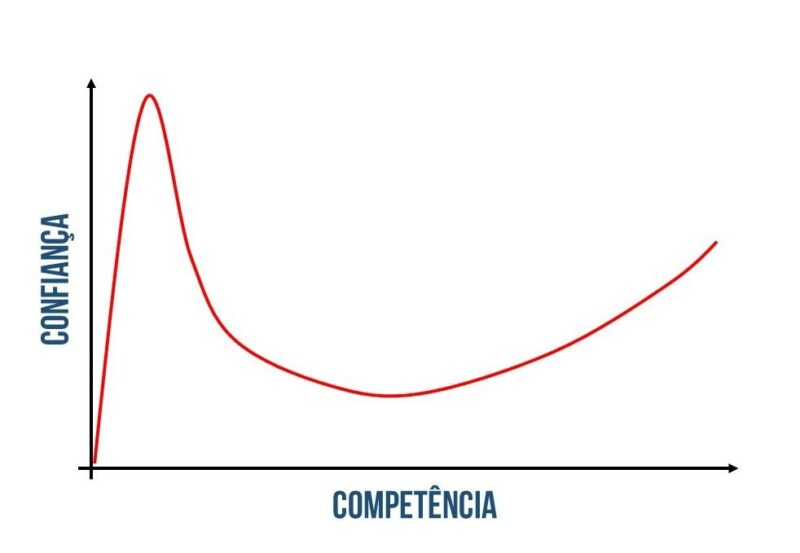
\includegraphics[scale=0.3]{figs/dk.jpeg} 
  		\caption*{O efeito Dunning Kruger. Não deixe que o primeiro pico te desmotive!}
	\end{figure}

	\newpage
	Falando de comandos agora - vamos começar com os básicos, isto é, aqueles que você usa todo dia só que de forma gráfica
	em programas como o Explorador do Windows. Tomando o Ubuntu Linux como referência, começamos nossa jornada no mundo CLI
	procurando um aplicativo chamado \textbf{Terminal}. Ao clicar nele, você irá se deparar com algo assim: 
	
	\vspace{1ex}
	\texttt{user@linux: ~}
	\vspace{1ex}

	O que significa que a pessoa usuária de nome \texttt{user} está, ou "at" em inglês, (\texttt{@}) no computador de nome
	\texttt{linux}. Depois dos dois pontos, irão aparecer os comandos que você digitar. Tais comandos serão interpretados pela
	\textit{shell} - um programa que roda "por trás das cortinas" e analisa os comandos para saber se são válidos ou não.

	Dado esse contexto, podemos começar a usar o computador com o poder da CLI. Geralmente, a primeira coisa que se faz ao 
	entrar no computador é saber onde você está. 
	
	\subsubsection{Onde estou? O pwd}
	Para descobrir sua localização no sistema de arquivos, digite \texttt{pwd} e pressione Enter. Esse comando vêm de 
	\textit{print working directory}, o que traduz, a grosso modo, para "mostre o diretório no qual se está trabalhando". O
	resultado esperado é um caminho ou \textit{path} como \texttt{/home/user}. 

	Isso indica que você está na pasta pessoal, ou "lar", de \texttt{user}. Essa pasta, por sua vez, está 
	na coleção de "lares" das pessoas que usam o sistema (\texttt{/home}). Por fim, essa coleção é só mais uma pasta no que 
	se chama de \textbf{raiz} do sistema de arquivos, representada por um \texttt{/}. 

	\subsubsection{O que eu tenho? O ls} 

	Agora que você sabe onde está, como descobrir o que tem em cada pasta? Para isso, use o comando \texttt{ls}. Isso deve
	retornar a \textit{lista} de arquivos e pastas que estão dentro do diretório no qual está trabalhando. Por exemplo, em um sistema
	de uso pessoal, é esperado que \texttt{/home/user} tenha pastas como \texttt{Videos, Downloads, Imagens, Musica}, entre
	outras. 
	
	\subsubsection{Mudança de diretório. O cd} 

	Você também vai querer entrar e sair de demais pastas durante seu trabalho no computador. O comando de \textit{change
	directory}, \texttt{cd}, permite a navegação no sistema. Para acessar a pasta um nível acima da qual você está, use 
	\texttt{cd ..} 


	Caso o diretório esteja na mesma pasta em que você se encontra, simplesmente adicione o nome desta depois do comando. 
	Por exemplo, \texttt{cd Videos} te leva aos seus vídeos. Você pode, também, ir para um \textit{local qualquer} no sistema
	de arquivos digitando seu \textit{path}. Para acessar uma pasta com programas instalados, use seu caminho como 
	\textbf{argumento} do comando. Por exemplo: 
	
	\vspace{1ex}
	\texttt{cd /usr/bin} 
	\vspace{1ex}

	\subsubsection{Entrada e saída (I/O)}

	Aqui, trataremos de comandos que fazem \textit{writes}, ou "escritas", e, portanto, entram e saiem com \textit{bytes} em disco. 

	\paragraph{Criação de arquivo:} 
	\paragraph{}
	Para gerar um arquivo de tipo qualquer, use o \texttt{touch}: 
	
	\begin{enumerate} 
		\item{Arquivo de texto: \texttt{touch Documentos/meuTexto.txt}} 
		\item{Arquivo de vídeo: \texttt{touch ../meuVideo.mp4}}
		\item{Arquivo de imagem: \texttt{touch /porDoSol.png}}
		\item{Arquivo qualquer: \texttt{touch arquivoGenerico}}
	\end{enumerate}

	\paragraph{Copiando arquivos:} 
	\paragraph{} 
	O comando \texttt{cp} permite que você copie arquivos de um lugar para outro. Vejamos seu uso: 
	\begin{enumerate} 
		\item{Copiando um arquivo: \texttt{cp Documentos/meuTexto.txt .}}
		\item{Copiando uma pasta: \texttt{cp -R Videos Documentos}}
	\end{enumerate} 


	Tá, temos coisas novas aqui. Primeiramente, repare que o comando toma dois parâmetros. O primeiro é 
	o caminho do objeto \textit{a ser copiado}, enquanto que o segundo é o caminho \textit{para onde} ele será copiado. 
	
	Em segundo lugar, veja no caso 1 que copiei o arquivo de texto \texttt{meuTexto.txt} da pasta \texttt{Documentos} 
	para o diretório no qual \textit{atualmente estou}. Se lembra que \texttt{..} representa a pasta um nível acima
	na hierarquia? Então, um ponto sozinho simboliza a pasta na qual você está trabalhando. 
	
	Por fim, para copiar uma pasta passamos uma \textit{flag} para \texttt{cp} junto de seus argumentos. 
	A \textit{flag} \texttt{-R} funciona como um modificador do comando e, nesse caso, manda o \texttt{cp}
	copiar \textbf{recursivamente} o arquivo especificado, ou seja, o comando "entra" na pasta e copia o que
	tem dentro dela, \textbf{incluindo} a própria pasta. 

	
	\paragraph{Movendo arquivos}
	\paragraph{}

	Mover arquivos funciona de forma análoga ao \texttt{cp}, com uma diferença significativa sendo que não é necessário 
	especificar a \textit{flag} \texttt{-R} para mover pastas - basta usar o comando como se fossem arquivos ordinários. 

	\begin{enumerate} 
		\item{\texttt{mv Documentos DocumentosSecretos}} 
		\item{\texttt{mv Videos/meuVideo.mp4 Downloads}} 
		\item{\texttt{mv meuTexto.txt Downloads/curriculo.txt}} 
	\end{enumerate} 

	Aqui, temos 3 usos distintos do \texttt{mv}. Vejamos um por um. No primeiro, estamos \textit{renomeando} a pasta de 
	nome \texttt{Documentos} para \texttt{DocumentosSecretos}, a qual está no diretório no qual se está trabalhando. 


	Em segundo lugar, de fato movemos o arquivo \texttt{meuVideo.mp4} na pasta Videos para a pasta Downloads. Repare, no 
	entanto, que caso a pasta Downloads \textbf{não} existisse, o arquivo de vídeo seria "convertido" em um arquivo 
	genérico de nome \texttt{Downloads}, o que acarretaria uma \textit{perda de informação} grave. Por mais óbvio que isso
	seja, certifique-se de que o destino para o qual quer mover seus dados realmente exista. 


	Finalmente, juntamos os dois casos acima em um terceiro. Aqui, movemos o arquivo \texttt{meuTexto.txt}, presente na pasta
	atual, para a pasta Downloads \textbf{e} renomeamos o arquivo para \texttt{curriculo.txt}. Fizemos duas tarefas em um 
	só comando. Esse é apenas um exemplo trivial de como é possível aumentar sua produtividade usando a CLI. 
	
	\paragraph{Apagando arquivos} 
	\paragraph{} 

	Essa seção requer atenção especial devido a possíveis catástrofes que podem acontecer no sistema. A não ser que você 
	configure-o ou utilize pacotes/programas adicionais para criá-lo, o conceito de lixeira, presente em sistemas
	como Windows e MacOS, \textbf{não existe} na linha de comando de SOs \textit{Unix-like} como Linux. 


	Em essência, a lixeira nada mais é do que uma pasta especial, na qual os dados ficam indefinidamente até que a pessoa
	utilizando o computador possa avaliar se os quer ou não. Nesse sentido, no mundo do CLI, para colocar algo na lixeira,
	faríamos: 
	
	\vspace{1ex} 
	\texttt{mv arquivoIndesejado /caminho/para/a/lixeira} 
	\vspace{1ex} 

	Mas isso não é nada prático. Poderíamos usar um apelido, ou \textit{alias}, para tornar o comando acima algo menor 
	como \texttt{lixo}, mas este recurso será tratado em breve. No meio tempo, pode-se simplesmente apagar,
	\textbf{de forma irreversível}, um dado arquivo. 

	Para isso, vamos \textit{remover} o arquivo usando \texttt{rm}. A sintaxe é bem simples: 
	\begin{enumerate} 
		\item{\texttt{rm textoIndesejado.txt}} 
		\item{\texttt{rm -r pastaIndesejada}} 
		\item{\texttt{rm -i videoPotencialmenteIndesejado}} 
	\end{enumerate}

	Novamente, temos 3 casos. Nos dois primeiros, apagamos um arquivo de texto e, no segundo, apagamos uma pasta usando 
	a \textit{flag} recursiva \texttt{-r}. A terceira opção é mais segura, uma vez que a \textit{flag} \texttt{-i} trata a ação de forma
	interativa. O que isso quer dizer é que quando você clicar Enter para apagar, o sistema irá retornar uma mensagem 
	pedindo que você confirme sua ação com um sim ou não. Geralmente, isso se dá assim:
	
	\vspace{1ex}
	\texttt{rm: remove regular file?} 
	\vspace{1ex} 
	
	Para o qual você digita \texttt{y} ou \texttt{n} para sim ou não, respectivamente. 

	\subsection{Visualizando arquivos. O cat} 

	Vamos tratar de uma ferramenta muito útil para visualizar arquivos de texto. Veja, o comando \texttt{cat} abre 
	\textit{qualquer} tipo de arquivo para visualização. No entanto, abrir arquivos que não de texto irá renderizar 
	uma visualização esquisita em algo parecido com hexadecimal.

	\begin{figure}[ht!]
  		\centering
		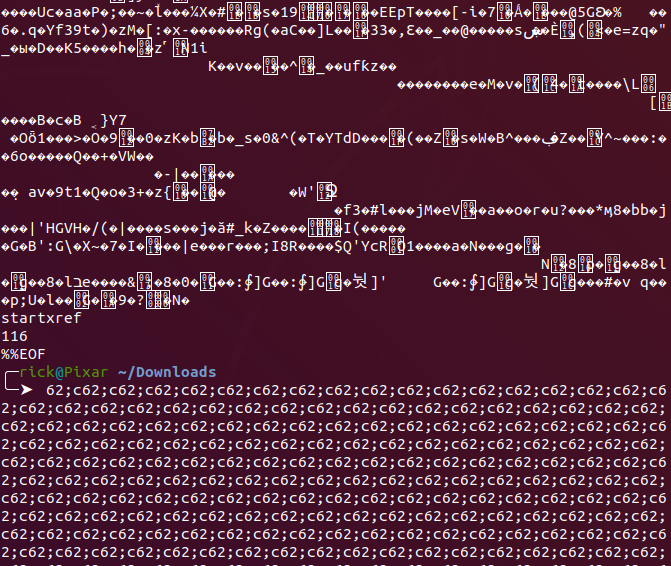
\includegraphics[scale=0.3]{figs/brokenCat.png} 
  		\caption*{Visualização quebrada de um PDF utilizando o cat}
	\end{figure}


	Por outro lado, executar o comando em um arquivo de texto normal, irá mostrar corretamente seu conteúdo. 
	Suponha que você tenha um arquivo chamado \texttt{listaDeCompras} estruturado da seguinte forma:

	\begin{enumerate}
		\item{Banana}
		\item{Laranja} 
		\item{Livro de Álgebra Linear} 
		\item{Leite desnatado} 
		\item{Cubo mágico} 
	\end{enumerate} 

	Rodar \texttt{cat listaDeCompras} irá lhe mostrar uma lista estruturada exatamente igual da forma como você a escreveu. 
	Note que desde que o arquivo seja de texto, sua visualização será idêntica. O que isso significa é que caso você receba um 
	arquivo de texto do Windows, isto é, terminado em \texttt{.txt} e e ele estiver em um formato universal no qual 
	seu computador trabalha como UTF-8 ou ASCII e não estiver corrompido, sua visualização será igual a de um arquivo 
	de texto do Linux. Para visualizá-lo: 

	\vspace{1ex}
	\texttt{cat textoDoWindows.txt} 
	\vspace{1ex} 

	\subsection{Editando textos} 

	O assunto edição de textos no terminal é extenso e vai além do que esse livro propõe. Ainda assim, vou lhe mostrar como abrir 
	um arquivo de texto e começar a editá-lo. Imagine que você queira escrever a lista do tópico anterior em um arquivo chamado 
	\texttt{compras.txt}. Para isso, você faria: 
	
	\vspace{1ex} 
	\texttt{nano compras.txt} 
	\vspace{1ex}

	Entenda que \texttt{nano} não é exatamente um "comando" como estamos tratando aqui. Ele é apenas um dos inúmeros 
	programas de edição de texto CLI que existem. Fiz referência a ele devido à sua fácil utilização, mas existem
	outras opções mais configuráveis como o \texttt{emacs}, o \texttt{vim} (meu preferido) e o \texttt{micro}. 

	\newpage

	\section{Python} 

	Nessa seção iremos iniciar a tratar do assunto \textbf{programação de computadores}. No contexto desse livreto, 
	irei defini-la como escrever \textit{scripts}, traduzindo literalmente como "roteiros", que instruem o computador a fazer
	determinada(s) ação(ões). Como estamos em um nível iniciante, a melhor linguagem de programação para essa tarefa 
	é o Python. 

	\subsection{Contexto técnico} 

	A linguagem Python é \textit{interpretada}, o que significa que o código escrito por você \textbf{não} é "empacotado" e
	convertido em binário (0s e 1s que o computador lê em nível fundamental) como ocorre em linguagens \textit{compiladas}. 
	Isso gera um certo \textit{overhead} ("atraso") de performance para o programa ao mesmo tempo que proporciona grande 
	flexibilidade à linguagem. Sua natureza flexível, com o uso de \textbf{módulos}, é um dos pontos que fizeram Python 
	tão popular na computação moderna. 

	\subsection{Instalando módulos. O pip}

	Para tirar proveito dessas "extensões" da linguagem, devemos incluí-las em seu interpretador. Para tanto, vamos usar
	o gerenciador de pacotes nativo do Python para baixar os módulos diretamente do \href{https://pypi.org/}{PyPI}.
	Esse programa se chama \texttt{pip} e pode ser invocado diretamente da linha de comando: 

	\vspace{1ex}
	\texttt{pip install módulo1 módulo2 módulo3 ...} (1)
	\vspace{1ex} 

	Caso esteja usando um sistema Linux atual, é esperado que o \texttt{pip} já esteja instalado no sistema (assim como o Python). 
	Caso contrário, instale-o pelo próprio terminal. Em sistemas Ubuntu/Debian, você faria: 

	\vspace{1ex} 
	\texttt{sudo apt install python python-pip} (2)
	\vspace{1ex} 

	e digitaria sua senha de usuário. Em seguida, tente reinstalar os módulos pelo \texttt{pip}. Note, contudo, que rodar o comando 
	(1) irá instala-los no interpretador \textbf{global} do Python. Isso não é exatamente um problema, mas na maior 
	parte dos casos, é tido como uma má prática porque você pode querer trabalhar com o mesmo módulo de diferentes versões,
	podem acontecer problemas com determinadas versões/dependências e a técnica que vou mostrar em seguida deixa seu trabalho
	mais organizado. 

	\begin{figure}[ht!]
  		\centering
		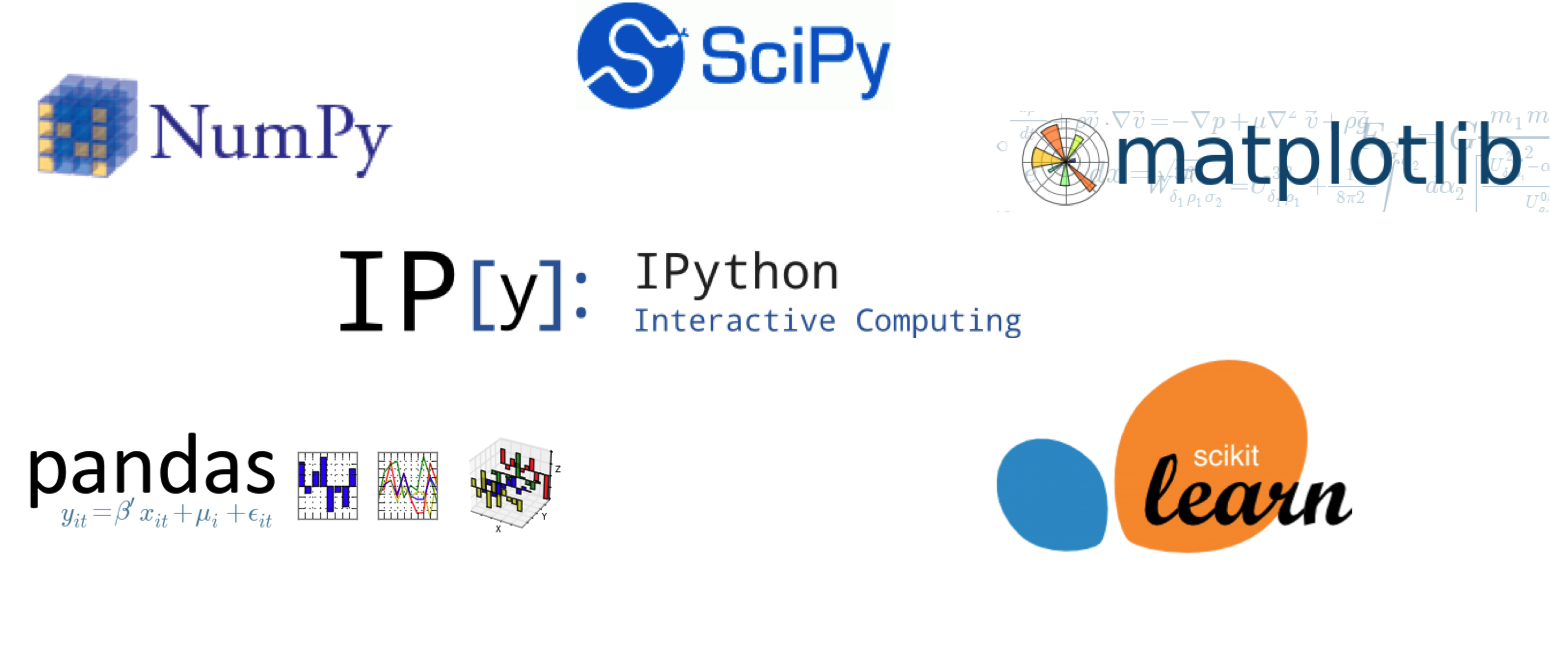
\includegraphics[scale=0.2]{figs/modules.png} 
  		\caption*{Alguns dos módulos mais populares de Python}
	\end{figure}

	\newpage

	\subsection{Ambiente virtual. O venv} 

	Para solucionar esse "problema", as pessoas desenvolvedoras por trás do Python vieram com um conceito chamado ambiente
	virtual, o qual pode ser criado utilizando um módulo nativo da linguagem, espertamente chamado de \texttt{venv} para 
	\textit{Virtual Environment}.

	Suponha que você desenvolva um aplicativo de cálculo numérico e quer torná-lo disponível em seu site para uso público.
	Você poderia logar em seu servidor com SSH e criar um ambiente na sua \textit{home} que irá conter o aplicativo. 
	Vamos criá-lo: 
	
	\vspace{1ex}
	\texttt{python -m venv calculoNumerico} 
	\vspace{1ex} 

	Veja aqui que passei a \textit{flag} \texttt{-m} para o interpretador, uma vez que não estou apenas invocando o interpretador Python,
	mas um módulo específico para criação de \textit{venvs}. Esse módulo, por sua vez, recebe um argumento que é o nome do 
	ambiente virtual.

	Agora existe uma pasta chamada \texttt{calculoNumerico} em seu diretório atual, a qual pode ser acessada usando \texttt{cd}. 
	Ao entrar na pasta do \textit{venv}, você ainda \textbf{não} estará propriamente no ambiente. Veja, usando \texttt{ls},
	que existem algumas sub-pastas como \texttt{bin, include, lib, lib64} e um arquivo \texttt{pyenv.cfg}. O que aconteceu aqui
	é que agora existe um "mini Python" nessa pasta, e você pode adicionar, mover e apagar pastas e arquivos à vontade dentro
	do diretório do \textit{venv} sem afetar a instalação global. 

	\subsubsection{Ativando o ambiente} 

	Para propriamente "entrar" no \textit{venv}, você deve carregar uma configuração específica para a sua \textit{shell}. 
	Essa configuração está na forma de um script dentro da pasta \texttt{bin} do ambiente virtual e pode ser carregada usando o 
	comando \texttt{source}. Então, dentro da pasta de seu \textit{venv}, faça:

	\vspace{1ex}
	\texttt{source bin/activate}
	\vspace{1ex} 

	o que irá ativar o ambiente virtual. A partir de agora, podemos instalar os pacotes usando \texttt{pip} e eles estarão
	isolados da instalação global do Python. 

	\vspace{1ex} 
	\texttt{(calculoNumerico) pip install numpy Flask pandas} 
	\vspace{1ex} 

	Isso irá instalar módulos para computação numérica (\texttt{numpy}), \textit{backend} (\texttt{Flask}) e
	análise de dados (\texttt{pandas}) no ambiente virtual de nome \texttt{calculoNumerico}. Após editar e executar todos
	os arquivos necessários, saia do ambiente virtual simplesmente digitando \texttt{deactivate} no terminal. 


\end{document}

%\section{Git}

